\documentclass{beamer}

\usepackage{verbatim}
\usepackage{fancyvrb}
\usepackage{amsmath}
\usepackage{mathtools}
\usepackage{booktabs}
\usepackage{amssymb}
\usepackage{graphicx}
\usepackage{calc}
\usepackage{color}
\usepackage{multicol}
\usepackage{wrapfig}
\usepackage{natbib}
\usepackage[ruled,vlined]{algorithm2e}
\usepackage{animate}
\usepackage{mathtools}
\usepackage{listings}

\usepackage{cmbright}
\fontencoding{OT1}\fontfamily{cmbr}\selectfont %to load ot1cmbr.fd
\DeclareFontShape{OT1}{cmbr}{bx}{n}{% change bx definition
<->cmbrbx10%
}{}
\normalfont % back to normalfont

% two col: two columns
\newenvironment{twocol}[4]{
\begin{columns}[c]
\column{#1\textwidth}
#3
\column{#2\textwidth}
#4
\end{columns}
}

\makeatletter
\setbeamertemplate{theorem begin}
{%
\begin{\inserttheoremblockenv}
  {}{\usebeamerfont*{block title}\usebeamercolor[fg]{block title}%
  \inserttheoremname
  %\inserttheoremnumber
  \ifx \inserttheoremaddition \empty \else\ (\inserttheoremaddition)\fi
  \inserttheorempunctuation}
  \normalfont
  }
  \setbeamertemplate{theorem end}{\end{\inserttheoremblockenv}}
\makeatother

\newcommand{\E}{\mathrm{E}}
\newcommand{\Var}{\mathrm{Var}}
\newcommand{\Cov}{\mathrm{Cov}}
\newcommand{\sd}{\mathrm{sd}}
\newcommand{\s}{\mathrm{s}}
\newcommand{\Corr}{\mathrm{Corr}}
\newcommand{\rank}{\mathrm{rank}}
\newcommand{\trace}{\mathrm{trace}}
\newcommand{\nullspace}{\mathrm{null}}
\newcommand{\myspan}{\mathrm{span}}
\DeclareMathOperator*{\argmax}{arg\,max}
\DeclareMathOperator*{\argmin}{arg\,min}
\DeclareMathOperator*{\softmax}{softmax}

\definecolor{darkgreen}{rgb}{0,0.5,0}

\newtheorem{proposition}[theorem]{Proposition}
\newtheorem{exe}{Exercise}
\newtheorem{notation}{Notation}
\newtheorem{remark}{Remark}

\definecolor{darkgreen}{rgb}{0,0.5,0}

\title{Model Diagnostics}
\author{Zhenisbek Assylbekov}
\institute{Department of Mathematics}
\date{Regression Analysis}

\AtBeginSection[]
{
  \begin{frame}<beamer>
    \tableofcontents[currentsection]
  \end{frame}
}

\begin{document}

\begin{frame}
  \titlepage
\end{frame}

\begin{frame}{Diagnostics we have already discussed}
\begin{itemize}
\item Residuals $e_i$ vs. 
\begin{itemize}
    \item $i$ (independence)
    \item $x_1$, \ldots , $x_k$ (linearity)
    \item $\hat{Y}_i$ (linearity and homogeneity of variance)
\end{itemize} 
\item\pause Q-Q plot of $e_1$, \ldots , $e_n$.
\item\pause VIF$_j$ for $j = 1, \ldots, k$.
\item\pause Significance tests (Runs, Levene's, Shapiro-Wilk)
\item\pause Now we'll discuss 
\begin{itemize}
    \item added variable plots,
    \item leverages,
    \item DFFITS,
    \item Cook's distance.
\end{itemize}
\end{itemize}
\end{frame}

\begin{frame}[fragile]{The problem with marginal plots}
\begin{center}
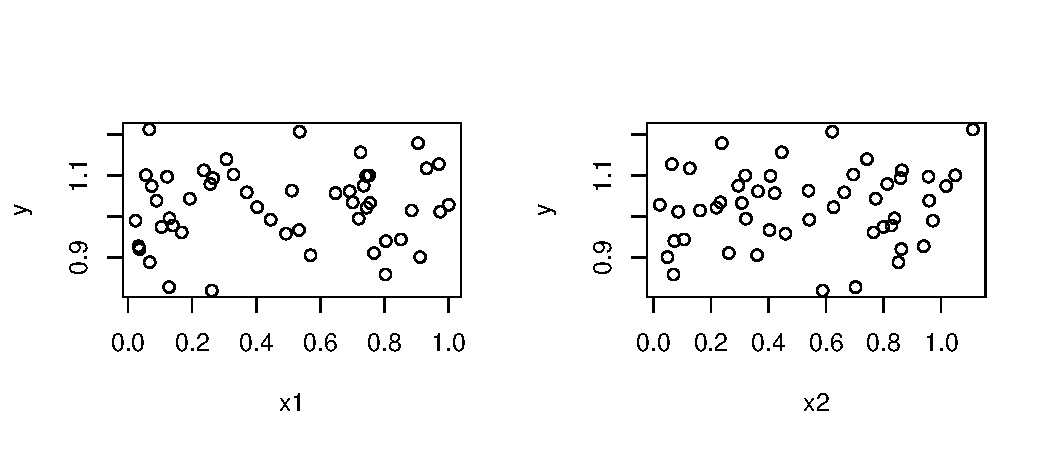
\includegraphics[height=.4\textheight]{plots/marginal.pdf}    
\end{center}
\pause No dependence b/w $Y$ and $x_j$ marginally, but significant association jointly:
\begin{footnotesize}
\pause\begin{verbatim}
            Estimate Std. Error t value Pr(>|t|)    
(Intercept)  0.05083    0.07726   0.658    0.514    
x1           0.95536    0.07651  12.487   <2e-16 ***
x2           0.96312    0.07658  12.576   <2e-16 ***
\end{verbatim}
\end{footnotesize}
\end{frame}

\section{Added variable plots}

\begin{frame}{Problems with marginal plots}
\begin{small}
\begin{itemize}
\item Residuals $e_i$ versus a predictor values $x_i,j$ can show whether $x_j$ may need to be transformed or whether we should add a quadratic term $x_j^2$.
\item\pause We can omit the predictor  from the model and plot the residuals versus the predictor to see if the predictor explains residual variability.
\item\pause However these plots can also be misleading: \pause e.g., we can have
\vspace{-5pt}
\begin{center}
    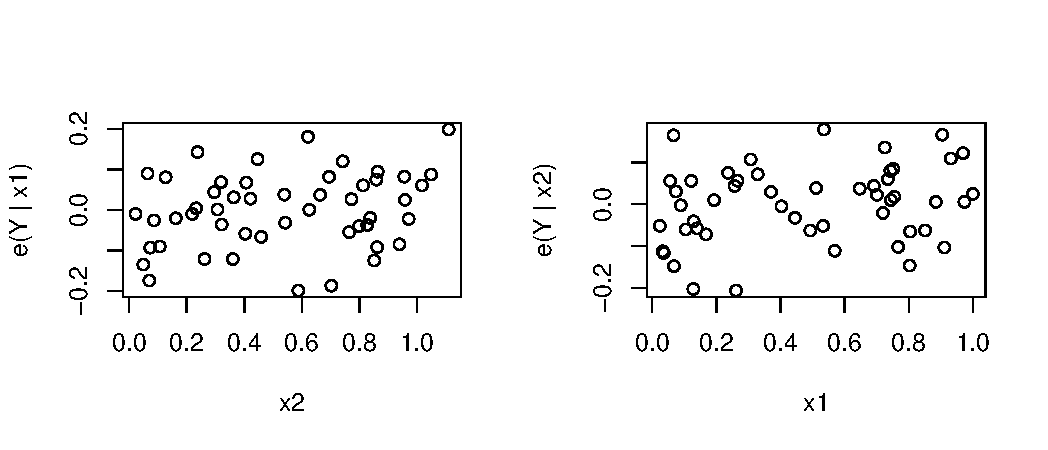
\includegraphics[height=.3\textheight]{plots/res-xj.pdf}
\end{center}
where $e(Y\mid x_j)$ are residuals when we regress $Y$ on $x_j$ only.
\end{itemize}
\end{small}
\end{frame}

\begin{frame}[fragile]{Added variables plots}
\begin{itemize}
    \item The previous plots suggest that $x_2$ is not needed when $x_1$ is in the model, \pause or that $x_1$ is not needed when $x_2$ is in the model.
    \item\pause But we still have significance for both $x_1$ and $x_2$ when they are \textit{simultaneously} in the model!
    \begin{footnotesize}
    \begin{verbatim}
                Estimate Std. Error t value Pr(>|t|)    
(Intercept)  0.05083    0.07726   0.658    0.514    
x1           0.95536    0.07651  12.487   <2e-16 ***
x2           0.96312    0.07658  12.576   <2e-16 ***
    \end{verbatim}
    \end{footnotesize}
    \item\pause An \textbf{added variable plot} tries to fix this problem.
    \item\pause It answers the question: Does $x_j$ explain any \textit{residual} variability once the rest of the predictors are in the model?
\end{itemize}
\end{frame}


\begin{frame}{10.1 Added variable plots}
\begin{itemize}
\item Consider a pool of predictors $x_1 , \ldots, x_k$. Let’s consider predictor $x_j$ where $j = 1, \ldots, k$.
\item\pause Regress $Y_i$ vs. all predictors except $x_j$, call the residuals $e_i(Y\mid\mathbf{x}_{-j})$.
\item\pause Regress $x_j$ vs. all predictors except $x_j$, call the residuals $e_i(x_j\mid\mathbf{x}_{-j})$.
\item\pause The added variable plot for $x_j$ is $e_i(Y\mid\mathbf{x}_{-j})$ vs. $e_i(x_j\mid\mathbf{x}_{-j})$.
\item\pause If you fit a simple linear regression
$$
e_i(Y\mid\mathbf{x}_{-j}) = \beta_j\cdot e_i(x_j\mid\mathbf{x}_{-j})+\epsilon_i
$$
then the LSE $\hat\beta_j$ \textit{is the same} as one would get from fitting the full model $Y_i = \beta_0 + \beta_1 x_{i1} + \cdots + \beta_k x_{ik} + \epsilon_i$. 
\item\pause Gives an idea of the functional form of $x_j$: a transformation in $x_j$ should mimic the pattern seen in the plot. %; the methods of Section 3.9 apply.
\end{itemize}
\end{frame}

\begin{frame}{10.1 Added variables plots illustration}
Let's go back to our synthetic example:

\vspace{-10pt}

\begin{center}
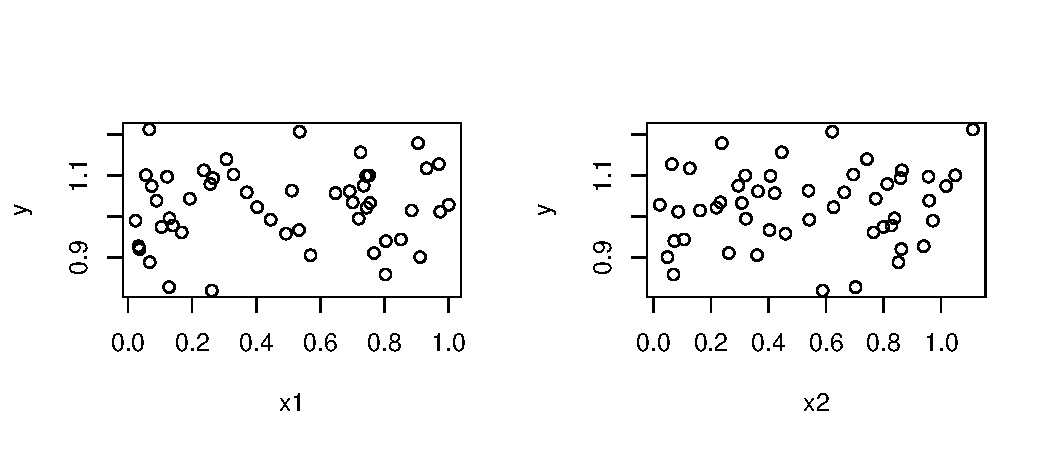
\includegraphics[height=.4\textheight]{plots/marginal.pdf}
\end{center}

\pause 
\begin{center}
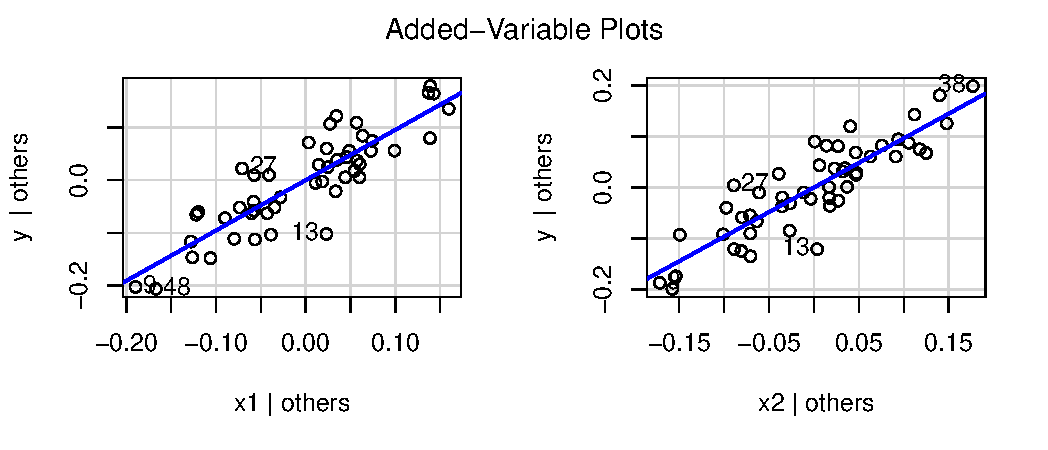
\includegraphics[height=.4\textheight]{plots/av_plots.pdf}
\end{center}

\end{frame}


\begin{frame}[fragile]
\frametitle{Salary data, first order terms only}
\begin{scriptsize}
\begin{verbatim}
> head(salary_data)
  salary age educ pol
1     38  25    4   D
2     45  27    4   R
3     28  26    4   O
4     55  39    4   D
5     74  42    4   R
6     43  41    4   O
> m = lm(salary ~ ., data=salary_data)
> summary(m)

Coefficients:
            Estimate Std. Error t value Pr(>|t|)    
(Intercept)  17.0313     7.3459   2.318  0.03735 *  
age           0.8983     0.1968   4.565  0.00053 ***
educ          1.5039     1.1841   1.270  0.22632    
polO        -16.5404     4.8807  -3.389  0.00484 ** 
polR          9.1587     4.8482   1.889  0.08139 .  
---

Residual standard error: 8.209 on 13 degrees of freedom
Multiple R-squared:  0.8374,	Adjusted R-squared:  0.7873 
\end{verbatim}
\end{scriptsize}
\end{frame}

\begin{frame}{Added variable plots}
\centerline{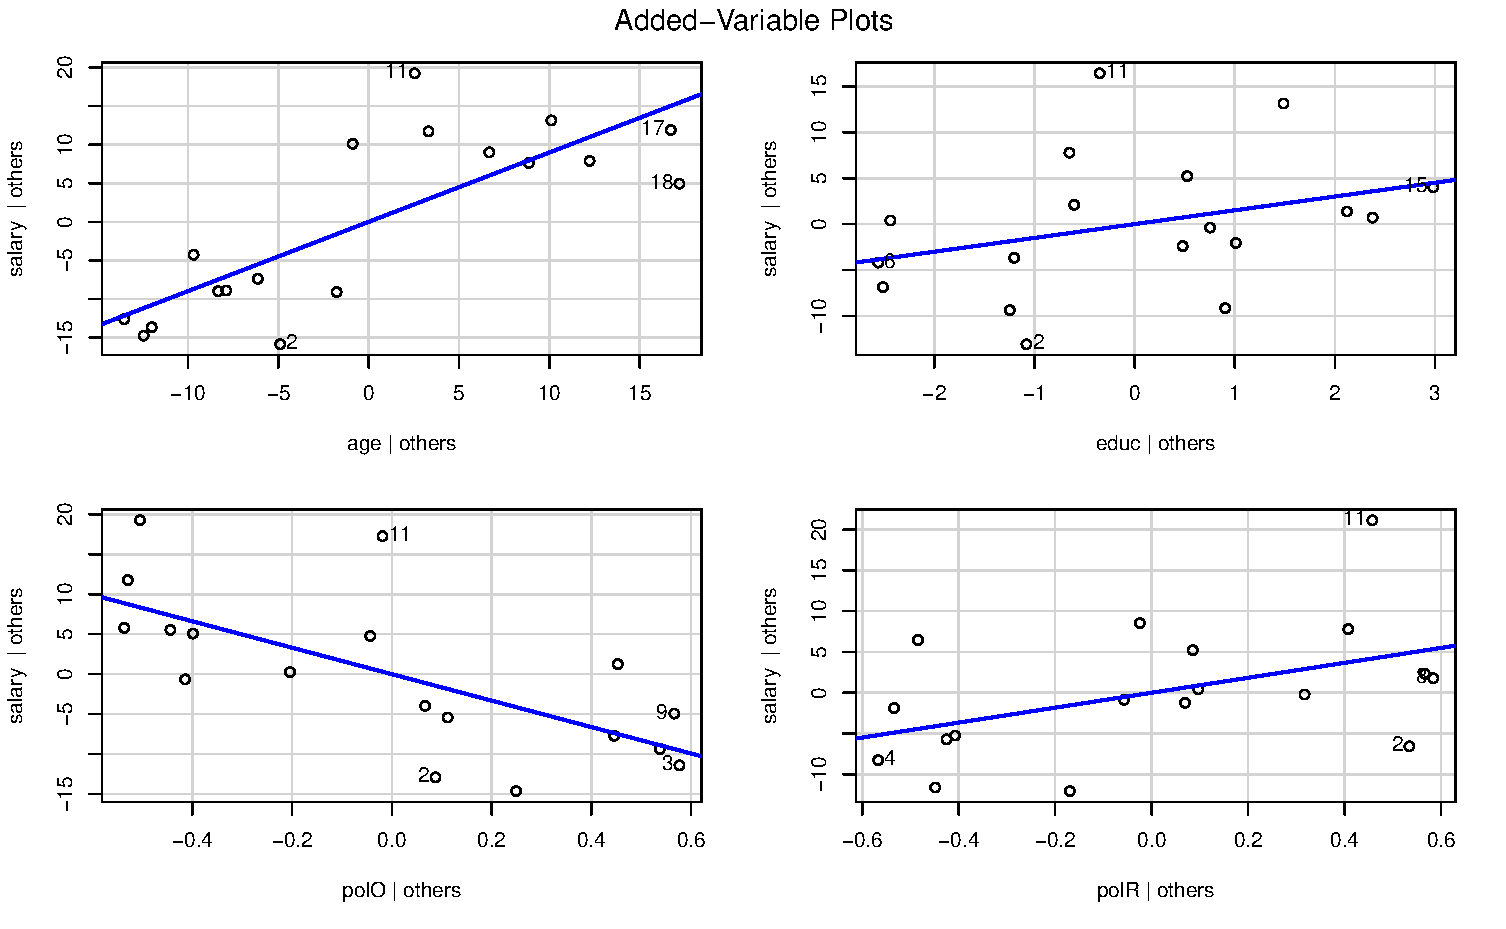
\includegraphics[height=0.7\textheight]{plots/salary_av.pdf}}

\pause Age effect is nonlinear; let's add a quadratic term.
\end{frame}

\begin{frame}[fragile]
\frametitle{Salary data, quadratic effect in age}
\begin{verbatim}
> m1 = lm(salary ~ . + I(age^2), data=salary_data)
> summary(m1)

Coefficients:
              Estimate Std. Error t value Pr(>|t|)    
(Intercept) -39.224169  16.810142  -2.333 0.037839 *  
age           3.463723   0.740666   4.676 0.000535 ***
educ          2.166475   0.883369   2.453 0.030453 *  
polO        -15.455108   3.571147  -4.328 0.000983 ***
polR         10.118144   3.544586   2.855 0.014500 *  
I(age^2)     -0.028831   0.008166  -3.530 0.004143 ** 
---

Residual standard error: 5.984 on 12 degrees of freedom
Multiple R-squared:  0.9202,	Adjusted R-squared:  0.887 
\end{verbatim}
\end{frame}

\begin{frame}{Added variables plots w/ quadratic age}
\centerline{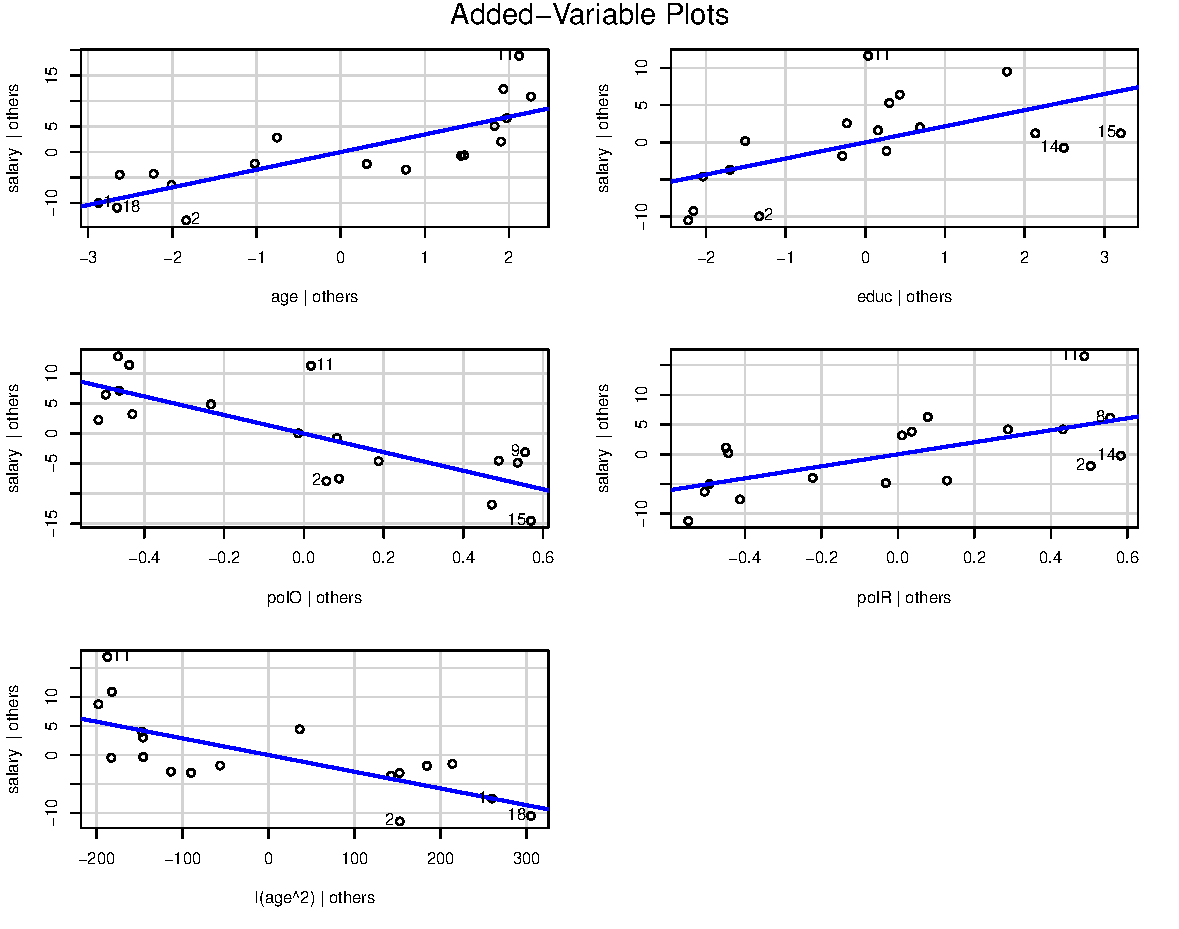
\includegraphics[width=.75\textwidth]{plots/salary_av2.pdf}}
Education is now significant! \pause The incorrect
functional form for age was \textit{masking} the
importance of education.
\end{frame}

\begin{frame}[fragile]
\frametitle{Salary data, quadratic effect in education}
\begin{footnotesize}
\begin{verbatim}
> summary(m2)

Call:
lm(formula = salary ~ . + I(age^2) + I(educ^2), data = salary_data)

              Estimate Std. Error t value Pr(>|t|)    
(Intercept) -75.977348  18.262402  -4.160 0.001589 ** 
age           2.787032   0.626151   4.451 0.000977 ***
educ         18.751324   5.739109   3.267 0.007501 ** 
polO        -13.976910   2.848879  -4.906 0.000467 ***
polR          9.495127   2.790631   3.403 0.005903 ** 
I(age^2)     -0.018677   0.007298  -2.559 0.026558 *  
I(educ^2)    -1.342341   0.461108  -2.911 0.014161 *  
---

Residual standard error: 4.697 on 11 degrees of freedom
Multiple R-squared:  0.9549,	Adjusted R-squared:  0.9304 
\end{verbatim}
\end{footnotesize}
\end{frame}


\begin{frame}{Added variable plots w/ quad. age and educ}
\begin{center}
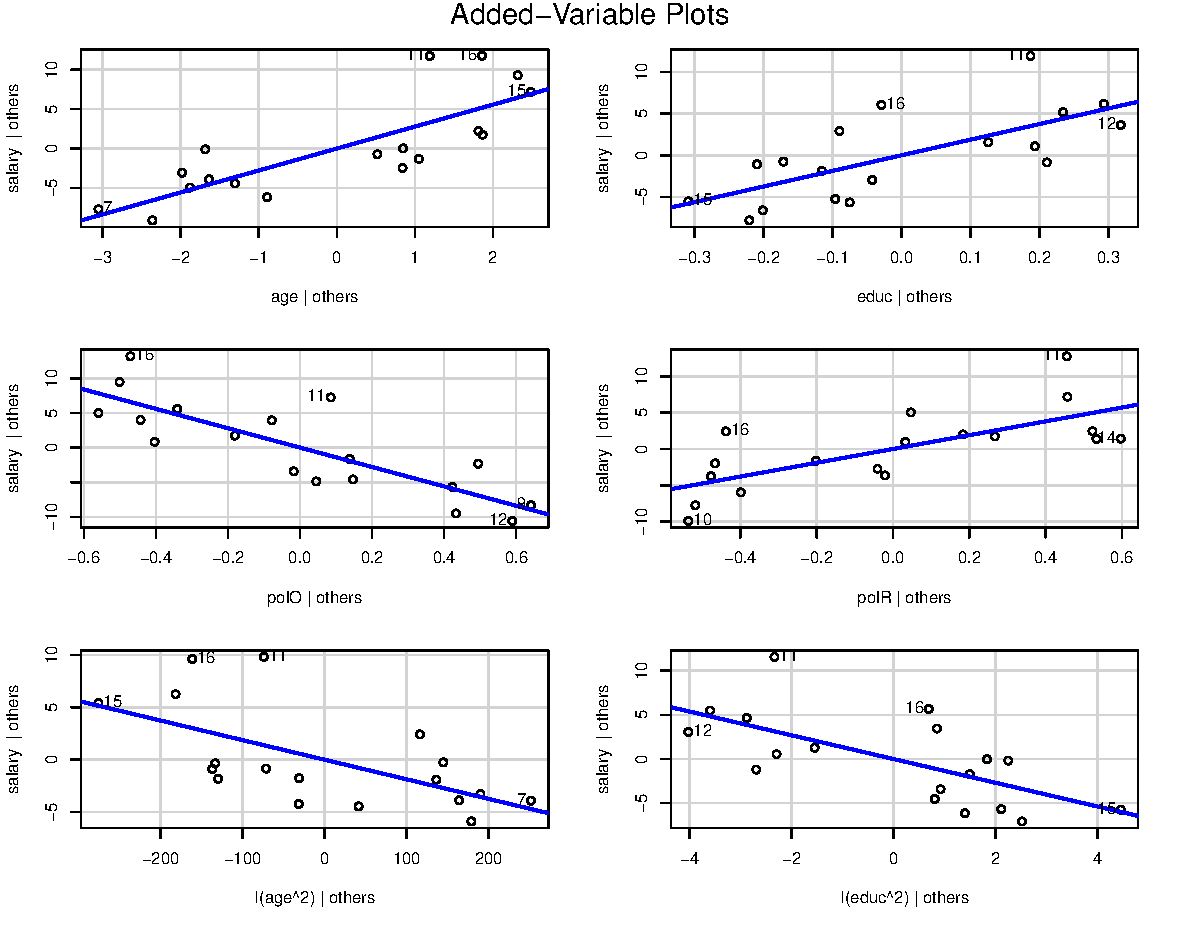
\includegraphics[height=.85\textheight]{plots/salary_av3.pdf}        
\end{center}
\end{frame}

\section{Outliers, leverages, DFFITs, Cook's distance}

\begin{frame}{Outliers}
\begin{itemize}
\item Outliers are data points which are ``far away'' from the bulk of data. \pause Observations may be outlying 
\begin{itemize}
    \item relative to predictors, i.e. $\mathbf{x}_i$ relative to other $\{\mathbf{x}_j\}_{j\ne i}$
    \item\pause relative to the model, i.e. $Y_i$ relative to $\hat{Y}_i$.
\end{itemize} 
\item\pause \textbf{Studentized deleted residuals} are designed to detect outlying $Y_i$ observations; \textbf{leverages} detect outlying $\mathbf{x}_i$ points.
\item\pause Outliers have the potential to influence the fitted regression
function:
\begin{itemize}
\item\pause if the outlying points follow the modeling
assumptions and are representative, they may \textit{strengthen} inference and reduce error in predictions 
\item\pause if not, outlying values may skew inference a lot and yield
models with poor predictive properties.
\end{itemize}
\end{itemize}
\end{frame}

\begin{frame}{Outliers \& influential points}
\begin{itemize}
\item Often outliers are flagged and deemed suspect as mistakes
or observations not gathered from the same population as the other observations.
\item\pause Outliers are sometimes of interest in their own right and may illustrate aspects of the dataset that require more careful study.
\item\pause Although an observation may be flagged as an outlier, the
point \textit{may or may not} affect the fitted regression function
more than other points.
\item\pause A \textbf{DFFIT} is a measure of influence that an individual point
$(\mathbf{x}_i, Y_i)$ has on the regression surface at $\mathbf{x}_i$.
\item\pause \textbf{Cook's distance} is a consolidated measure of influence the point $(\mathbf{x}_i, Y_i)$ has on the regression surface at all $n$ points $\mathbf{x}_1, \ldots, \mathbf{x}_n$.
\end{itemize}
\end{frame}

\begin{frame}{Variance of $\hat{Y}_i$}
Recall that 
\begin{itemize}
    \item $\hat{\mathbf{Y}}=\pause\mathbf{X}\hat{\boldsymbol\beta}$,
    \item\pause $\hat{\boldsymbol\beta}\pause=(\mathbf{X}^\top\mathbf{X})^{-1}\mathbf{X}^\top\mathbf{Y}$,
    \item\pause $\mathbf{Y}\pause\sim\mathcal{N}_n(\mathbf{X}\boldsymbol\beta,\sigma^2\mathbf{I}_n)$
\end{itemize} 
Thus,
\begin{align*}
\onslide<7->{\Cov[\hat{\mathbf{Y}}]}\onslide<8->{&=\Cov[\mathbf{X}\hat{\boldsymbol\beta}]}\onslide<9->{=\Cov[\mathbf{X}(\mathbf{X}^\top\mathbf{X})^{-1}\mathbf{X}^\top\mathbf{Y}]\\}
\onslide<10->{&=\Cov[\mathbf{HY}]=\mathbf{H}\Cov[\mathbf{Y}]\mathbf{H}^\top=\mathbf{H}\sigma^2\mathbf{IH}^\top\\}
\onslide<11->{&=\sigma^2\mathbf{H}}
\end{align*}
\onslide<12->{$\Rightarrow$\,\,
$\Var[\hat{Y}_i]=\sigma^2h_{ii}$, and its unbiased estimator is $\text{MSE}\cdot h_{ii}$.}

\end{frame}


\begin{frame}{10.2 Studentized deleted residuals}
\begin{itemize}
\item The \textbf{standardized residuals}
$$
r_i=\frac{Y_i-\hat{Y}_i}{\sqrt{\text{MSE}(1-h_{ii})}}
$$
have a constant variance of 1.
\item\pause Typically, $|r_i|>2$ is considered ``large.''
\item\pause $h_{ii}=\mathbf{x}^\top_i(\mathbf{X}^\top\mathbf{X})^{-1}\mathbf{x}_i$ is called the $i^\text{th}$ \textbf{leverage value}.
\item\pause A refinement of the standardized residual that has a recognizable distribution is the \textbf{studentized deleted residual}
$$
t_i=\frac{Y_i-\hat{Y}_{i}}{\sqrt{\text{MSE}_{(i)}(1-h_{ii})}}
$$
where $\text{MSE}_{i(i)}$ is obtained from the model when $i$-th example was removed from the data.
\end{itemize}
\end{frame}

\begin{frame}{Studentized deleted residuals}
\begin{itemize}
\item In fact, no need to fit $n$ additional regressions, because there is relationship b/w MSE and MSE$_{(i)}$:
$$
(n-p)\text{MSE}=(n-p-1)\text{MSE}_{(i)}+\frac{e_i^2}{1-h_{ii}}
$$
(prove it)

\item\pause Studentized deleted residuals are distributed as
$$
t_i\sim t_{n-p-1}.
$$
\item\pause Therefore, outlying $Y$-values may be flagged by using Bonferroni's adjustment and taking
$$
|t_i|>t_{1-\alpha/(2n); n-p-1}
$$
as outlying.
\item\pause Typically, in practice, one simply flags observations with $|t_i|>t_{1-\alpha/2; n-p-1}$ as \textit{possibly} outlying in consideration with other diagnostics.
\end{itemize}
\end{frame}

\begin{frame}{10.3 Leverage}
\begin{itemize}
\item The leverages $h_{ii}$ get larger the further the points $\mathbf{x}_i$ are from the mean $\bar{\mathbf{x}} = \frac1n\sum_{i=1}^n\mathbf{x}_i$, adjusted for ``how many'' other
predictors are in the vicinity of $\mathbf{x}_i$.
\item\pause Use the fact that $\mathbf{H} = \mathbf{X}(\mathbf{X}^\top\mathbf{X})^{-1}\mathbf{X}^\top = \mathbf{HH}$ to show $\sum_{i=1}^n h_{ii} = p$ and $0 \le h_{ii} \le1$.
\item\pause A large leverage $h_{ii}$ indicates that $\mathbf{x}_i$ is far away from the other predictors $\{\mathbf{x}_j\}_{j\ne i}$ \pause and that $\mathbf{x}_i$ may influence the fitted value $\hat{Y}_i$ more than other $x_j$'s will influence their respective fitted values. \pause This is evident in the variance of the residual $\Var[Y_i - \hat{Y}_i] = \sigma^2 \sqrt{1 - h_{ii}}$. The larger $h_{ii}$ is, the smaller
$\Var[Y_i - \hat{Y}_i]$ will be and hence the closer $\hat{Y}_i$ will be to $Y_i$ on average.
\item\pause The rule of thumb is that any leverage $h_{ii}$ that is larger than
twice the mean leverage $p/n$, i.e. $h_{ii} > 2p/n$, is flagged as
having ``high'' leverage.
\end{itemize}
\end{frame}

\begin{frame}[fragile]{Leverage}
\begin{itemize}
\item Note that the leverages $h_{ii}$ depend only on the $\mathbf{x}_i$ and hence
indicate which points might \textit{potentially} be influential.
\item \pause (p. 400) When making predictions $\mathbf{x}_{n+1}$ at a point not in the
data set, we consider the measure of distance of this point from the points $\mathbf{x}_1 , \ldots, \mathbf{x}_n$ given by $h_{n+1} = \mathbf{x}_{n+1}(\mathbf{X}^\top\mathbf{X})^{-1}\mathbf{x}_{n+1}$.
\item \pause If $h_{n+1}$ is much larger than any of the $\{h_{11}, \ldots, h_{nn}\}$ you may
be extrapolating far outside the general region of your data.
\item \pause In \texttt{R}, you can get leverages using \verb|hatvalues| command.
\end{itemize}
\end{frame}

\begin{frame}{10.4 DFFITs}
\begin{itemize}
\item The $i^\text{th}$ DFFIT, denoted DFFIT$_i$, is given by
$$
\text{DFFIT}_i=\frac{\hat{Y}_i-\hat{Y}_{i(i)}}{\sqrt{\text{MSE}_{(i)}h_{ii}}}=t_i\sqrt{\frac{h_{ii}}{1-h_{ii}}},
$$
\pause where $\hat{Y}_i$ is fitted value of regression surface (calculated using all $n$ observations) at $\mathbf{x}_i$ and $\hat{Y}_{i(i)}$ is fitted value of regression surface \textit{omitting the point} $(\mathbf{x}_i, Y_i)$ at the point $\mathbf{x}_i$.
\item\pause $\text{DFFIT}_i$ is standardized distance between \textit{fitted} regression surfaces \textit{with} and \textit{without} the point $(\mathbf{x}_i, Y_i)$.
\item\pause Rule of thumb that $\text{DFFIT}_i$ is ``large'' when $|\text{DFFIT}_i|>1$ for small to medium-sized data sets and $|\text{DFFIT}_i|>2\sqrt{p/n}$ for large data sets. \pause We will often just note those $\text{DFFIT}_i$'s that are considerable larger than the bulk of the $\text{DFFIT}_i$'s.
\end{itemize}
\end{frame}

\begin{frame}{10.4 Cook's distance}
\begin{itemize}
\item The $i^\text{th}$ Cook's distance, denoted $D_i$, is an aggregate measure of the influence of the $i^\text{th}$ observation on all $n$ fitted values:
$$
D_i=\frac{\sum_{j=1}^n(\hat{Y}_j - \hat{Y}_{j(i)})^2}{p\cdot\text{MSE}}
$$
\pause This is the sum of squared distances, at each $\mathbf{x}_j$, between fitted regression surface calculated with all $n$ points and fitted regression surface calculated with the $i^\text{th}$ case removed, standardized by $p\cdot \text{MSE}$.
\item \pause Look for values of Cook's distance significantly larger than other values; these are cases that have disproportionate
influence on the fitted regression surface as a whole.
\end{itemize}
\end{frame}

\section{Review of Diagnostics}

\begin{frame}{Review of diagnostics}
\begin{itemize}
\item \structure{Variance inflation factors} VIF$_j$ tell you which predictors are highly correlated with other predictors. If you have one or more VIF$_j>10$, you \text{may} want to eliminate some of the predictors.
\vspace{10pt}

\pause Multicollinearity affects the interpretability of the model, but does not indicate the model is ``bad'' in any way.
\vspace{10pt}

\pause An alternative approach that allows keeping correlated predictors is ridge regression (Chapter 11).

\item \structure{Deleted residuals} $t_i \sim t_{n-p-1}$, so you can formally define an outlier as being larger than $t_{1 - \alpha/(2n), n-p-1}$.
\end{itemize}
\end{frame}

\begin{frame}{Review of diagnostics}
\begin{itemize}
\item \structure{Residual plots}. Plots of $e_i$ or $t_i$ vs. $\hat{Y}_i$ and versus each $x_1, \ldots, x_k$ help assess (a) correct functional form, (b) constant
variance, and (c) outlying observations. %If an anomaly is apparent in any of these plots I may look at an added variable plot. If the number of predictors is small I may look at every added variable plot. 
They may also suggest a transformation for a predictor or two.
\begin{itemize}
\item\pause Heteroscedasticy can be corrected by transforming $Y$, or else
modeling the variance directly (Chapter 11).
\item\pause Constant variance but nonlinear patterns can be accommodated by introducing quadratic terms. 
\end{itemize}

\pause\structure{Added variable plots} help figure out functional form of predictors, and whether significance is being driven by one or two points only.
\end{itemize}
\end{frame}

\begin{frame}{Review of diagnostics}
\begin{itemize}
\item \textbf{DFFIT}$_i$ and \textbf{Cook's distance} $D_i$ tell you which observations
\textit{influence} the fitted model the most. Sometimes one or two points can drive the significance of a predictor.
\item\pause \textbf{Leverages} tell you which points \textit{can potentially} influence the fitted model. %Useful for finding ``hidden extrapolations'' via $h_{n+1}$.
%\item (pp.~404–405) DFBETA_{ij} tells you how much observation $i$ affects regression coefficient $j$. Useful to ``zoom in'' on where influential points are affecting the model. 
\item\pause A \textbf{normal Q-Q plot} of the residuals will indicate  departures from normality.
\item\pause A list of the studentized deleted residuals, leverages, and Cook's distances helps to determine outlying values that may
be transcription errors or data anomalies and also indicates those observations that affect the fitted regression surface as
a whole.
\end{itemize}
\end{frame}

\begin{frame}{Standard diagnostic plots}
\begin{itemize}
\item $t_i$ vs. $h_i$. Which observations are outlying in $\mathbf{x}$-direction, outlying in $Y$-direction, or both?
\item $D_i$ vs. $i$. Which observations grossly affect fit of regression surface?
\item $e_i$ vs. $\hat{Y}_i$ and $t_i$ vs. $\hat{Y}_i$. Constant variance \& linearity.
\item $Y_i$ vs. $\hat{Y}_i$; how well model predicts its own data. Better models have points close to line $y = x$.
\item Normal probability plot of the $e_1, \ldots, e_n$.
\item Histogram of $e_1, \ldots, e_n$.
\item Plots of $e_i$ vs. each predictor $x_1 , \ldots, x_k$.
\item One more plot that prof. Hanson never looks at.
\end{itemize}
\end{frame}

\section{Example}

\begin{frame}{An example of diagnostics}
\centerline{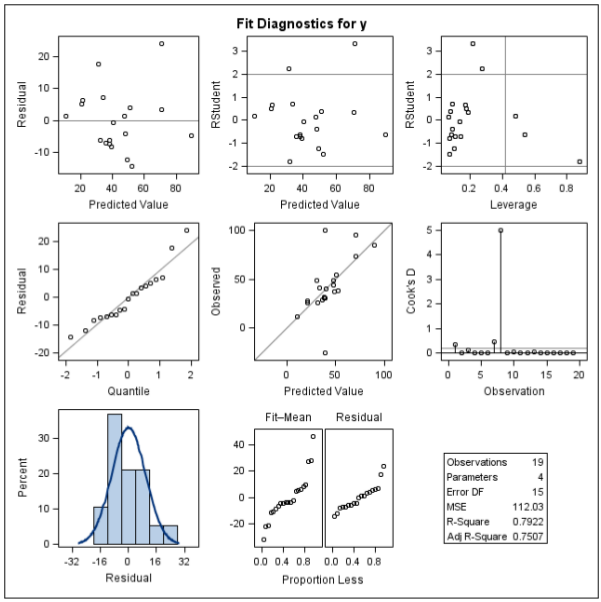
\includegraphics[height=.7\textheight]{plots/bp-diag}}
\vspace{10pt}
Model is $Y_i=\beta_0+\beta_1 x_{i1} + \beta_2 x_{i2} + \beta_{12} x_{i1} x_{i2} + \epsilon_i$. One highly influential point \& one poorly fit.
\end{frame}

\begin{frame}{Residual plots}
\centerline{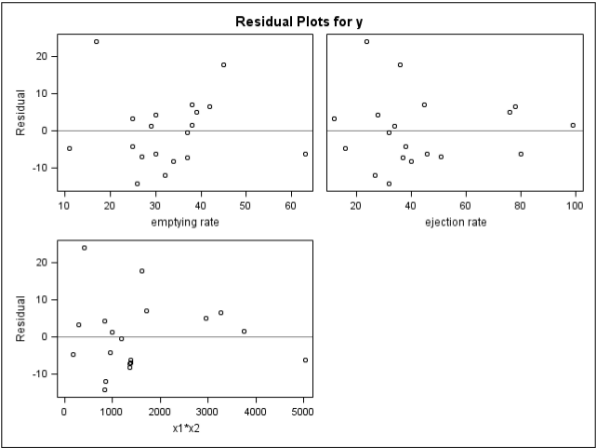
\includegraphics[scale=0.30]{plots/bp-res}}
\vspace{10pt}

These look pretty good, except for the one large residual.
\end{frame}

\begin{frame}{Arterial pressure data}
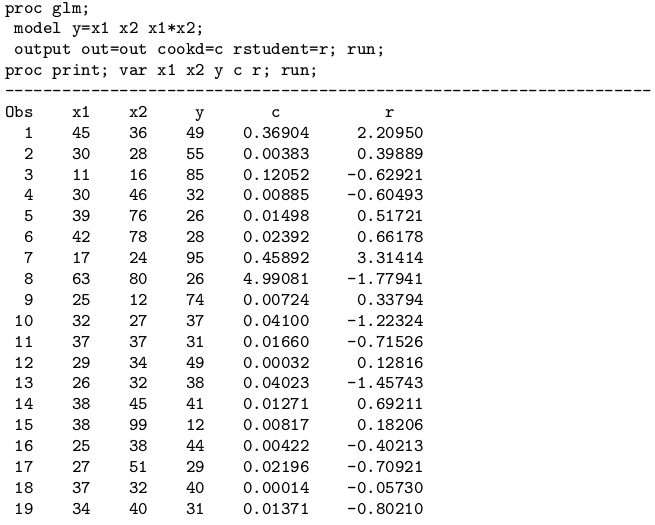
\includegraphics[scale=0.33]{plots/bp-cookd}
\vspace{10pt}

Obs. 7 has largest arterial pressure. Obs. 8 has relatively small arterial pressure.
\end{frame}

\begin{frame}{Dropping obs. 8 and obs. 7}
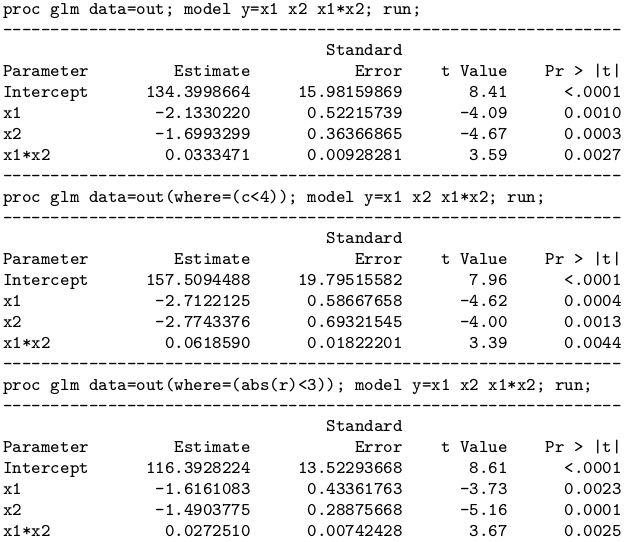
\includegraphics[scale=0.33]{plots/bp-two}
\vspace{10pt}

How do 7 and 8 affect the significance and/or magnitude of the effects?
\end{frame}

\end{document}